\section{recordtablemodel.cpp File Reference}
\label{recordtablemodel_8cpp}\index{recordtablemodel.cpp@{recordtablemodel.cpp}}
{\tt \#include $<$Qt\-Xml/qdom.h$>$}\par
{\tt \#include \char`\"{}main.h\char`\"{}}\par
{\tt \#include \char`\"{}treeitem.h\char`\"{}}\par
{\tt \#include \char`\"{}treemodel.h\char`\"{}}\par
{\tt \#include \char`\"{}appconfig.h\char`\"{}}\par
{\tt \#include \char`\"{}mainwindow.h\char`\"{}}\par
{\tt \#include \char`\"{}recordtabledata.h\char`\"{}}\par
{\tt \#include \char`\"{}recordtablemodel.h\char`\"{}}\par


Include dependency graph for recordtablemodel.cpp:\begin{figure}[H]
\begin{center}
\leavevmode
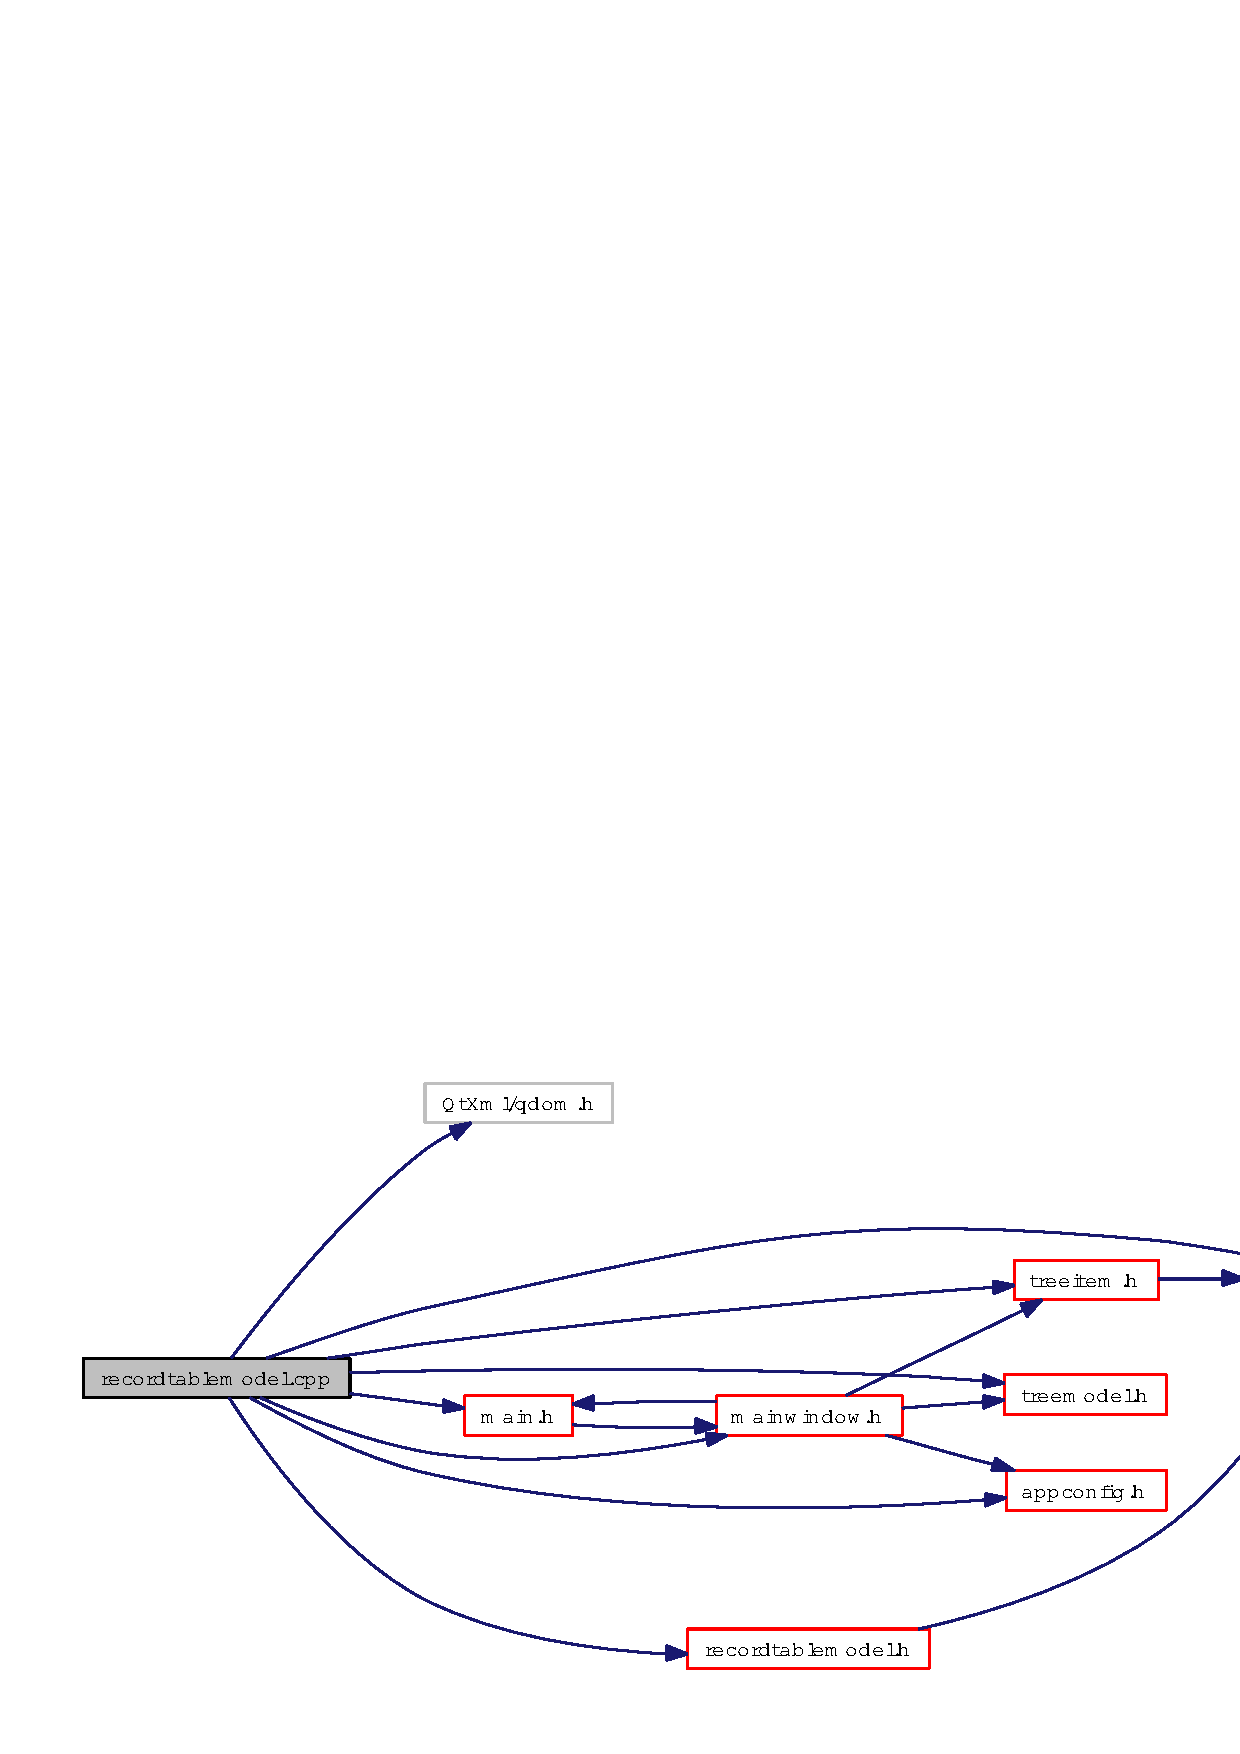
\includegraphics[width=354pt]{recordtablemodel_8cpp__incl}
\end{center}
\end{figure}
\subsection*{Variables}
\begin{CompactItemize}
\item 
{\bf appconfig} {\bf mytetraconfig}
\end{CompactItemize}


\subsection{Variable Documentation}
\index{recordtablemodel.cpp@{recordtablemodel.cpp}!mytetraconfig@{mytetraconfig}}
\index{mytetraconfig@{mytetraconfig}!recordtablemodel.cpp@{recordtablemodel.cpp}}
\subsubsection{\setlength{\rightskip}{0pt plus 5cm}{\bf appconfig} {\bf mytetraconfig}}\label{recordtablemodel_8cpp_69bd0a7d678d494effdef51808501712}




Definition at line 7 of file main.cpp.